\section{Neural Geometry Fields (NGFs)}\label{Sec:MainPart}

Sivaram and colleagues divide the Neural Geometry Fields pipeline into three distinct stages.

First, they input a base mesh \( \Sigma \) and partition it into quadrangular patches.
From this, they construct a trainable feature field \( \Psi : \Sigma \to \mathbb{R}^F \), associating each patch with a set of features that describe its surface properties, where each feature consists of \( F \) real components.
In the second stage, they feed these features, along with the 3D positions of the mesh, into a neural network that computes the displacement for each point on the mesh.
They then apply the displacements to the base mesh, producing a transformed conventional triangle mesh.
Finally, they optimize the feature field and patches using an inverse rendering algorithm.

In the following sections, we explore each stage in greater detail and provide an example to clarify the process further.






\subsection{Surface Partitioning into Patches}

Sivaram and colleagues introduce a method for surface representation by partitioning a simplified base mesh, denoted as \( \Sigma \), into quadrilateral patches \( \sigma \). 
To achieve this, they greedily merge adjacent triangles into near-rectangular quads. 
This process serves as a simplification step that reduces the mesh’s topological complexity, eliminates non-manifold configurations, and results in a more compact and regular representation of the surface geometry. 
By relying on quadrilateral patches rather than a purely triangular mesh, they decrease the overall number of patches and simplify the interpolation domain for later processing. 
\usetikzlibrary{calc, shapes.geometric, arrows.meta, decorations.pathreplacing}
\begin{figure}[ht]
  \centering
  \begin{adjustbox}{center}
  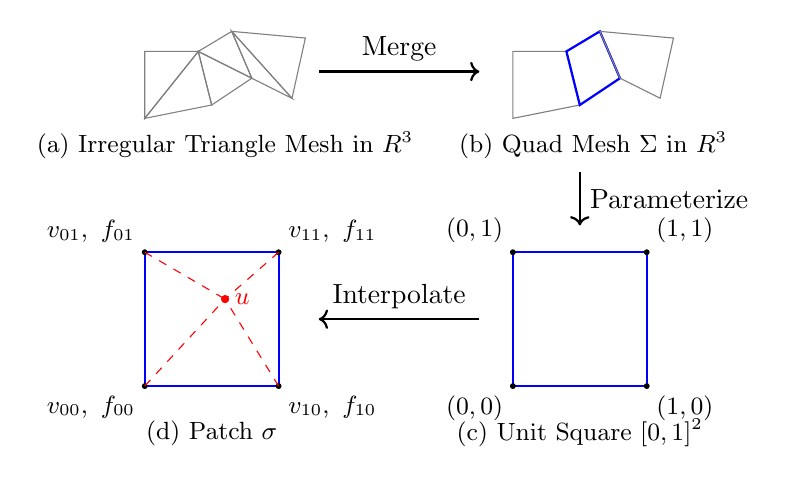
\begin{tikzpicture}[scale=0.85]

    % === Triangle Mesh (Left) ===
    \begin{scope}
      \coordinate (A) at (0,0);
      \coordinate (B) at (1,0.2);
      \coordinate (C) at (0.8,1);
      \coordinate (D) at (0,1);
      \coordinate (E) at (1.6,0.6);
      \coordinate (F) at (1.3,1.3);
      \coordinate (G) at (2.2,0.3);
      \coordinate (H) at (2.4,1.2);

      \draw[gray] (A) -- (B) -- (C) -- cycle;
      \draw[gray] (A) -- (C) -- (D) -- cycle;
      \draw[gray] (B) -- (E) -- (C) -- cycle;
      \draw[gray] (C) -- (E) -- (F) -- cycle;
      \draw[gray] (E) -- (G) -- (F) -- cycle;
      \draw[gray] (F) -- (G) -- (H) -- cycle;
      \node at (1.2, -0.4) {\small (a) Irregular Triangle Mesh in $\mathbb{R}^3$};
    \end{scope}

    % === Merge Arrow ===
    \draw[->, thick] (2.6,0.7) -- (5.0,0.7) node[midway, above] {Merge};

    % === Quadrilateral Mesh (Middle) ===
    \begin{scope}[xshift=5.5cm]
      \coordinate (A) at (0,0);
      \coordinate (B) at (1,0.2);
      \coordinate (C) at (0.8,1);
      \coordinate (D) at (0,1);
      \coordinate (E) at (1.6,0.6);
      \coordinate (F) at (1.3,1.3);
      \coordinate (G) at (2.2,0.3);
      \coordinate (H) at (2.4,1.2);

      \draw[gray] (A) -- (B) -- (C) -- (D) -- cycle;
      \draw[blue, thick] (B) -- (E) -- (F) -- (C) -- cycle; % highlighted patch
      \draw[gray] (E) -- (G) -- (H) -- (F) -- cycle;

      \node at (1.2, -0.4) {\small (b) Quad Mesh $\Sigma$ in $\mathbb{R}^3$};
    \end{scope}

    % === Down Arrow to Unit Square ===
    \draw[->, thick] (6.5,-0.8) -- (6.5,-1.6) node[midway, right] {Parameterize};

    % === Unit Square ===
    \begin{scope}[xshift=5.5cm, yshift=-4.0cm]
      \draw[blue, thick] (0,0) rectangle (2,2);
      \filldraw[black] (0,0) circle (1pt) node[anchor=north east] {\small $(0,0)$};
      \filldraw[black] (2,0) circle (1pt) node[anchor=north west] {\small $(1,0)$};
      \filldraw[black] (0,2) circle (1pt) node[anchor=south east] {\small $(0,1)$};
      \filldraw[black] (2,2) circle (1pt) node[anchor=south west] {\small $(1,1)$};
      \node at (1,-0.7) {\small (c) Unit Square $[0,1]^2$};
    \end{scope}

    % === Left Arrow to Feature Field ===
    \draw[->, thick] (5.0,-3) -- (2.6,-3) node[midway, above] {Interpolate};

    % === Feature Field (Right) ===
    \begin{scope}[yshift=-4.0cm]
      \draw[blue, thick] (0,0) rectangle (2,2);

      % Corner features (bold vectors), with f00 label moved outward
      \filldraw[black] (0,0) circle (1pt) node[anchor=north east] {\small $\bm{v_{00}},\ \bm{f_{00}}$};
      \filldraw[black] (2,0) circle (1pt) node[anchor=north west] {\small $\bm{v_{10}},\ \bm{f_{10}}$};
      \filldraw[black] (0,2) circle (1pt) node[anchor=south east] {\small $\bm{v_{01}},\ \bm{f_{01}}$};
      \filldraw[black] (2,2) circle (1pt) node[anchor=south west] {\small $\bm{v_{11}},\ \bm{f_{11}}$};

      % Interpolation point (u)
      \filldraw[red] (1.2,1.3) circle (1.5pt) node[right] {\small $\bm{u}$};

      % Lines from corners to interpolation point
      \foreach \x/\y in {0/0, 2/0, 0/2, 2/2} {
        \draw[dashed, red] (\x,\y) -- (1.2,1.3);
      }

      % Patch label
      \node at (1,-0.7) {\small (d) Patch $\sigma$};
    \end{scope}
    
  \end{tikzpicture}
  \end{adjustbox}
  \caption{Surface processing pipeline: The irregular triangle mesh is simplified and merged into a quadrilateral mesh $\Sigma$. A quadrilateral patch is extracted, which is then parameterized over the unit square $[0,1]^2$. This parameterization facilitates both geometric and feature field interpolation, with feature values interpolated at the patch's corners and at an arbitrary point $\bm{u}$. Inspired by~\cite{sivaram2024}.}
  \label{fig:surface_processing_pipeline}
\end{figure}
The initial mesh is simplified using QSlim, a robust simplification algorithm that preserves critical structures such as holes and intersections. 
After simplification, adjacent triangles are merged to form quadrilateral patches, producing a base mesh with a reduced patch count \( |Q| \) compared to a fully triangulated representation. 
This reduction compresses the mesh but also provides the base for an efficient and structured interpolation. 
Each patch \( \sigma \) is required to be diffeomorphic to the unit square \( [0,1]^2 \); that is, there must exist a smooth, bijective mapping with a smooth inverse between the patch and the square. 
This constraint ensures that interpolation across the patch is well-defined and invertible. 
The four corner vertices of each patch are mapped as follows: 
\[\begin{array}{c}
(0,0) \to v_{1,00}, 
(1,0) \to v_{1,10}, 
(0,1) \to v_{1,01}, 
(1,1) \to v_{1,11}.
\end{array}\]
To map an arbitrary point \( u = (u_x, u_y) \) within the unit square to its corresponding location on the surface patch \( \sigma \), bilinear interpolation is applied: 
\[\sigma(u) = (1 - u_y)((1 - u_x)v_{00} + u_x v_{10}) + u_y((1 - u_x)v_{01} + u_x v_{11}).\]
This two-stage interpolation first computes intermediate values along one axis (e.g., horizontal), then interpolates along the other axis (e.g., vertical). 
The result is a smooth and continuous surface across each quadrilateral patch. 
In this context, interpolation refers to estimating values at points within a patch based on the known values at its four corners. 
Bilinear interpolation smoothly blends these corner values to compute both positions and other properties (such as feature vectors) for any point inside the patch. 
This approach offers a simple and efficient way to represent complex surfaces using only a few key points. 
Beyond geometry, Sivaram et al. also interpolate scalar or vector-valued feature fields defined at the patch corners. 
Given feature values \( f_{00}, f_{10}, f_{01}, \) and \( f_{11} \), the interpolated feature value \( \Psi(u) \) at point \( u \) is calculated as: 

\[\Psi(u) = (1 - u_y)((1 - u_x)f_{00} + u_x f_{10}) + u_y((1 - u_x)f_{01} + u_x f_{11}).\]
This interpolation ensures that feature values vary smoothly across the surface, which is essential for effective learning in subsequent tasks. 
Features are represented as learnable, high-dimensional vectors attached to the corners of each quadrilateral patch. 
These feature vectors act as local descriptors, encoding important surface properties and guiding the neural network during the deformation process. 
The feature field \( \Psi \) assigns a vector in \( \mathbb{R}^F \) (where \( F \) is typically 32 or 64) to each point on the surface, interpolated from the patch corners. 
These features are optimized alongside the network parameters during training to accurately reconstruct the target surface geometry. 
The complete set of mesh vertices and their associated features is defined as: 
\[V = \bigcup_{\sigma} \{ v_{00}, v_{10}, v_{01}, v_{11} \}\]
\[F = \bigcup_{\sigma} \{ f_{00}, f_{10}, f_{01}, f_{11} \}.\]
Together, \( V \) and \( F \) describe the base geometry and the spatial distribution of features across the surface. 
Sivaram and colleagues feed this quadrilateral mesh and its associated features into a neural network, \( MLP_\theta \), which learns to refine the geometry while preserving the simplified base’s topology and structural properties.





%A regular formula

%\begin{equation}
%    x^2 + y^2 = z^2 
%\end{equation}
%and another one
%\begin{equation}
%    \left\Vert \vec{x} \right\Vert = \sqrt{\sum_{i=0}^{n}{x_i^2 + y_i^2}}.
%\end{equation}

%Here is something with matrices:
%\begin{equation}
%\bf{A}=
%\begin{bmatrix}
%    a & b & c\\
%    d & e & f\\
%\end{bmatrix}^\top.
%\end{equation}

%An some inline stuff $\sum a_i=\bf{B}$.

%\begin{table}
%    \caption[List of Symbols]{Keep a list of symbols in your paper.}
%    \label{tab:ListOfSymbols}
%    \resizebox{\columnwidth}{!}
%    {
%    \input{tabs/ListOfSymbols.tex}
%    }
%\end{table}